\chapter{Classification}
\newcommand{\linkAutoSklearnClassifier}{https://www.kaggle.com/andrewmvd/heart-failure-clinical-data}

Within auto-sklearn, we can make use of the \href{\linkAutoSklearnClassifier}{'AutoSklearnClassifier'\footnote{AutoSklearnClassifier: \href{\linkAutoSklearnClassifier}{\linkAutoSklearnClassifier}}} to implement a model for a classifcation problem.

\section{Heart Failure Prediction}

The first classification problem we discuss is about the prediction of heart failure based upon different parameters.

\subsection{Dataset}
\newcommand{\kagglelinkheartfailure}{https://www.kaggle.com/andrewmvd/heart-failure-clinical-data}

The \href{\kagglelinkheartfailure}{dataset\footnote{Heart Failure Prediction : \href{\kagglelinkheartfailure}{\kagglelinkheartfailure}}} can be found on Kaggle and contains 12 features which can be used to predict mortality by heart failure. Those features are:

\begin{itemize}
  \item age: The age of the person in the dataset.
  \item anaemia: Whether the person has decrease of red blood cells or hemoglobin ($boolean$).
  \item creatinine\_phosphokinase: The level of the CPK enzyme in the blood ($mcg/L$).
  \item diabetes: Whether the patient has diabetes ($boolean$).
  \item ejection\_fraction: The percentage of blood leaving the heart at each contraction ($percentage$).
  \item high\_blood\_pressure: Whether the patient suffers from hypertension ($boolean$).
  \item platelets: The number of platelets in the blood ($kiloplatelets/mL$).
  \item serum\_creatinine: The level of serum creatinine in the blood ($mg/dL$).
  \item serum\_sodium: The level of serum sodium in the blood ($mEq/L$).
  \item sex: woman or man ($binary$).
  \item smoking: Whether the patient smokes or not ($boolean$).
  \item time: Follow-up period ($days$)
\end{itemize}

\noindent There are 299 observations in the dataset. For none of the features data is missing.

\subsection{Model Performance}

To construct the model, we've taken 30\% out of the dataset for testing purposes. The remaining part will be used to build our model with a $random\_state$ of 42. After fitting the model with the training data we can measure the performance of the model on the training and testing data. On the training data the model scores an accuracy of 96,17\%.

The mean accuracy reduces for the testing data to 73,33\%. When we compare the actual testing labels with the predicitons of the model for the testing data, we get a accuracy score of 73,33\%, with a precision of 78,26\%

\begin{figure}[t]
  \begin{center}
    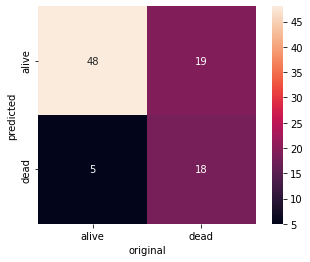
\includegraphics{heart-failure-heatmap}
    \caption{Heatmap plot of the confusion matrix}
  \end{center}
  % \centering
\end{figure}


\subsection{Model Comparision}

When we check the previous kaggle submissions with the same dataset, we can see the use of a LogisticRegression model from sklearn by '\href{https://www.kaggle.com/manthannagpurkar/heart-failure-prediction}{manthannagpurkar}' can improve the accuracy an the testing data up to 80\%.


\section{Diabetes Prediction}
\newcommand{\linkLogisticRegression}{https://scikit-learn.org/stable/modules/generated/sklearn.linear\_model.LogisticRegression.html}
\newcommand{\linkGaussianNB}{https://scikit-learn.org/stable/modules/generated/sklearn.naive\_bayes.GaussianNB.html?highlight=gaussiannb}
\newcommand{\linkRandomForestClassifier}{https://scikit-learn.org/stable/modules/generated/sklearn.ensemble.RandomForestClassifier.html?highlight=randomforestclassifier}



As a fourth model and a comparision with the outcome during the lectures, we've choosen the 'diabetes' dataset, which has been analysed by using a 'VotingClassifier' including a \href{\linkLogisticRegression}{LogisticRegression\footnote{\url{\linkLogisticRegression}}}, a \href{\linkGaussianNB}{GaussianNaiveBayes\footnote{\url{\linkGaussianNB}}} and a \href{\linkRandomForestClassifier}{RandomForestClassifier\footnote{\url{\linkRandomForestClassifier}}}. We will use the AutoSklearnClassifier and compare it's score with the VotingClassifier.

\subsection{Dataset}


\subsection{Model Performance}
\subsection{Model Comparision}
